%  !TeX  root  =  user_guide.tex

\section{Raster Terrain Modelling Plugin}

% when the revision of a section has been finalized, 
% comment out the following line:
%\updatedisclaimer

The Raster Terrain Modelling plugin can be used to calculate the slope, aspect, ruggedness, and
total curvature for digital elevation models (DEM). It is very simple to handle and provides an
intiuitive graphical user interface for creating new raster layers (See Figure
\ref{fig:raster_terrain_dialog}).
The plugin requires the following parameters to be specified before running:

\begin{itemize}[label=--]
\item \textbf{Analysis}: Can be one of slope, aspect, ruggedness, or total curvature
\item \textbf{Input layer}: Specify the input raster from a list of loaded
raster layers.
\item \textbf{Output layer}: Specify a name and path for the output raster file.
\item \textbf{Output format}: Specify a format type for the output raster file (Default is GeoTiff).
\end{itemize}

Slope: Calculates slope angle for each cell in degrees (based on first order derivative estimation).

Aspect: Exposition (starting with 0 for north direction, in degrees counterclockwise).

Ruggedness factor: A quantitative measurement of terrain heterogeneity.

Total curvature: A curvature measure that combines plan- and profile curvature.

\begin{figure}[ht]
   \centering
   \caption{Raster Terrain Modelling Plugin \nixcaption}\label{fig:raster_terrain_dialog}\smallskip
   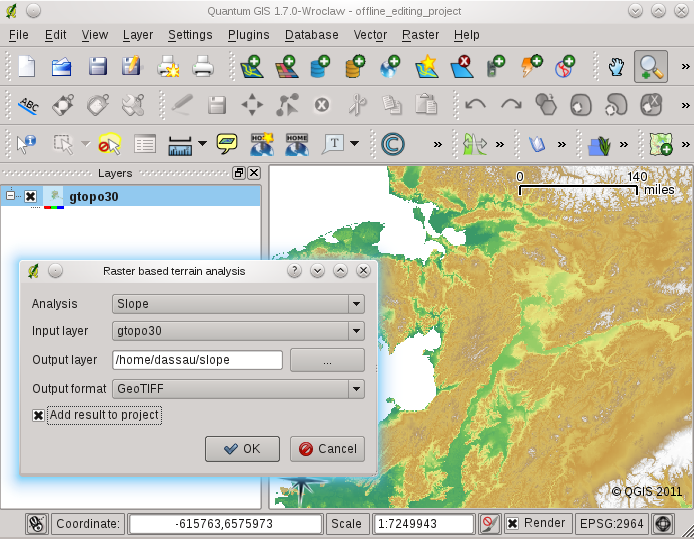
\includegraphics[clip=true, width=9cm]{raster_terrain_dialog}
\end{figure}

\minisec{Using the plugin}\label{raster_terrain_usage}

\begin{enumerate}
  \item Start QGIS and load a DEM raster layer. 
  \item Load the Raster Terrain Modelling plugin in the Plugin Manager (see Section 
  \ref{sec:load_core_plugin}) and click on the \toolbtntwo{raster_terrain}{Raster Terrain
Modelling} icon which appears in the QGIS toolbar menu. The Raster Terrain Modelling plugin dialog
appears as shown in Figure \ref{fig:raster_terrain_dialog}.
  \item Select an analysis method (e.g. \dropmenuopt{Slope}).
  \item Specify an output file
path, and an output file type.
  \item Click \button{Ok}.
\end{enumerate}
